%!TEX TS-program = xelatex
%!TEX engine = xelatex

\documentclass{standalone}

\usepackage{fontspec}
\setmainfont{Fira Mono}
\usepackage{unicode-math}
\setmathfont[Scale=MatchUppercase]{STIX Two Math}
\setmathrm[Scale=MatchUppercase,
           BoldFont=STIX Two Text Bold]{STIX Two Math}
\setmathtt[Scale=MatchUppercase]{Fira Mono}

\usepackage{tikz}

\begin{document}
  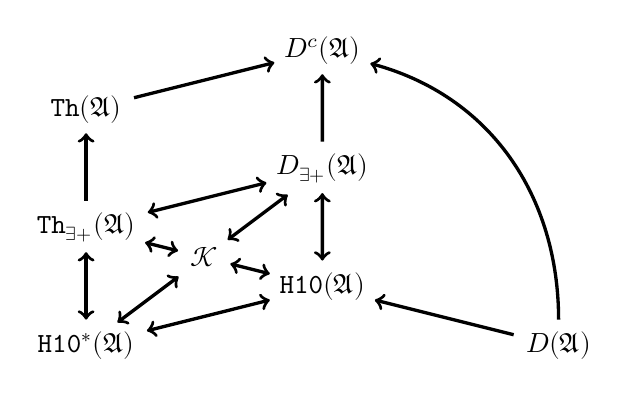
\begin{tikzpicture}[shorten >=1pt, scale=1.5]
  \tikzstyle{vertex}=[circle,fill=black!25,minimum size=17pt,inner sep=0pt]

  \path
    (0, 0) node (pdt) {\(\mathtt{H10}^*(\mathfrak{A})\)} --
    (0, 1) node (the) {\(\mathtt{Th}_{∃+}(\mathfrak{A})\)} --
    (0, 2) node (cth) {\(\mathtt{Th}(\mathfrak{A})\)} --
    (4, 0) node (ad) {\(D(\mathfrak{A})\)} --
    (2, 0.5) node (h10) {\(\mathtt{H10}(\mathfrak{A})\)} --
    (2, 1.5) node (de) {\(D_{∃+}(\mathfrak{A})\)} --
    (2, 2.5) node (cd) {\(D^c(\mathfrak{A})\)} --
    (1, .75) node (K) {\(\mathcal{K}\)};

  \foreach \f/\t in {cd/cth, cd/de, cth/the, h10/ad}
    \path[draw, very thick, <-]
      (\f) edge (\t);

  \foreach \f/\t in {the/pdt, de/h10, de/the, h10/pdt,
                     h10/K, K/de, the/K, pdt/K}
    \path[draw, very thick, <->]
      (\f) edge (\t);

  \draw[draw, very thick, <-, out=-15,  in=90]
    (cd) edge (ad);
  \end{tikzpicture}
\end{document}
